\section{Appendix}

\begin{figure}[!htb]
    \centering
    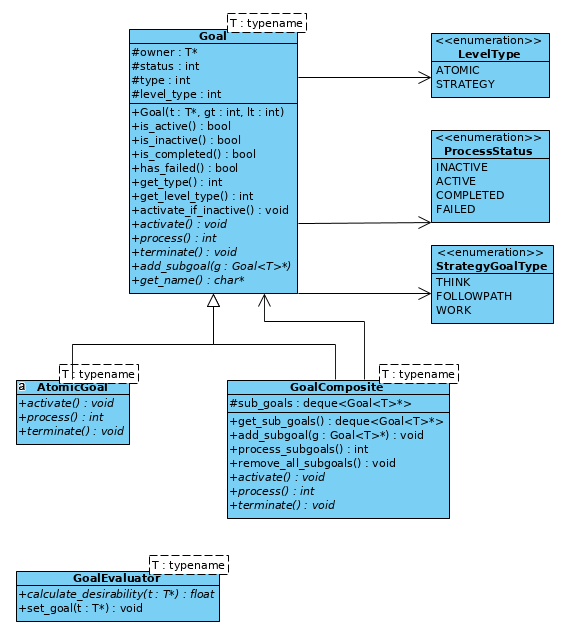
\includegraphics[scale=0.75]{res/Goal.jpg}
    \caption{The Goal<T> class.}\label{fig:goal}
\end{figure}

\begin{figure}[!htb]
    \centering
    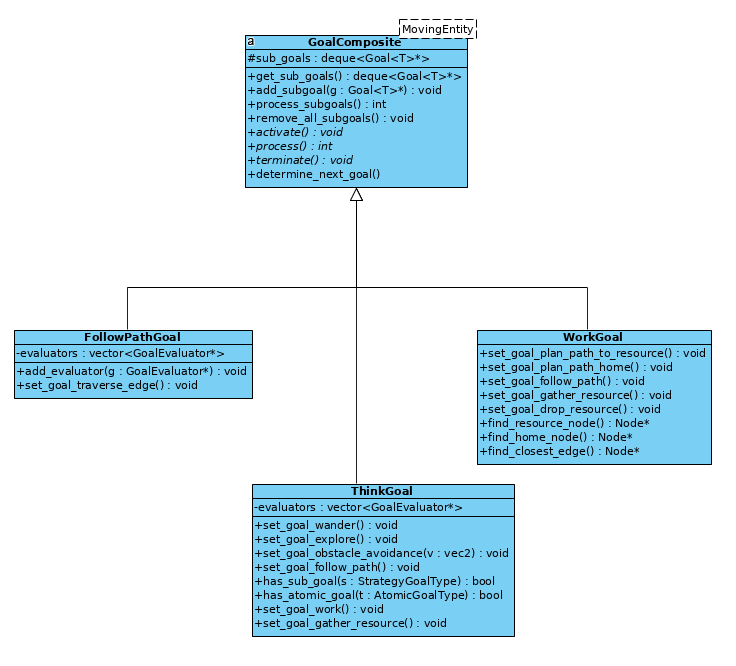
\includegraphics{res/GoalComposite-Inherit.jpg}
    \caption{GoalComposite Inheritance.}\label{fig:goalcomposite-inherit}
\end{figure}

\begin{figure}[!htb]
    \centering
    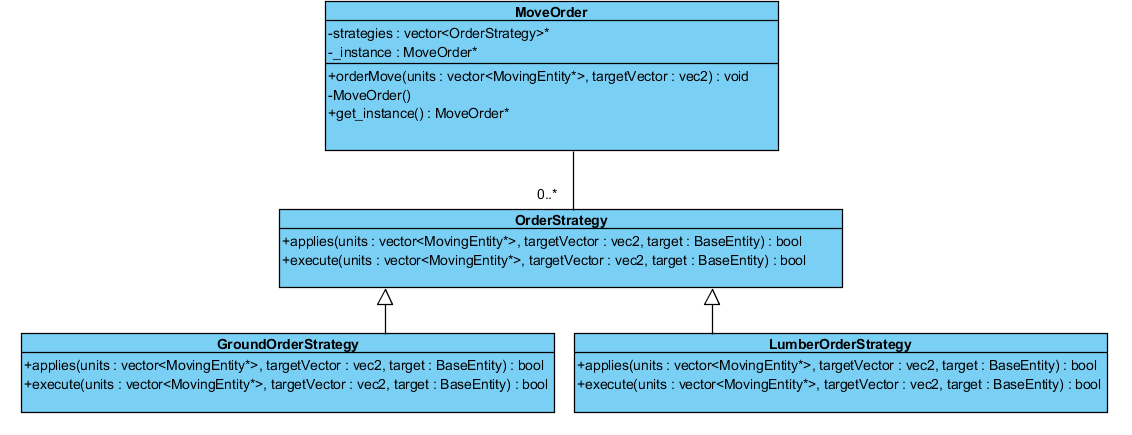
\includegraphics[angle=-90,origin=c,scale=0.65]
    {res/order-strategies.png}
    \caption{Order strategies}\label{fig:orderstrategies}
\end{figure}

\begin{figure}[!htb]
    \centering
    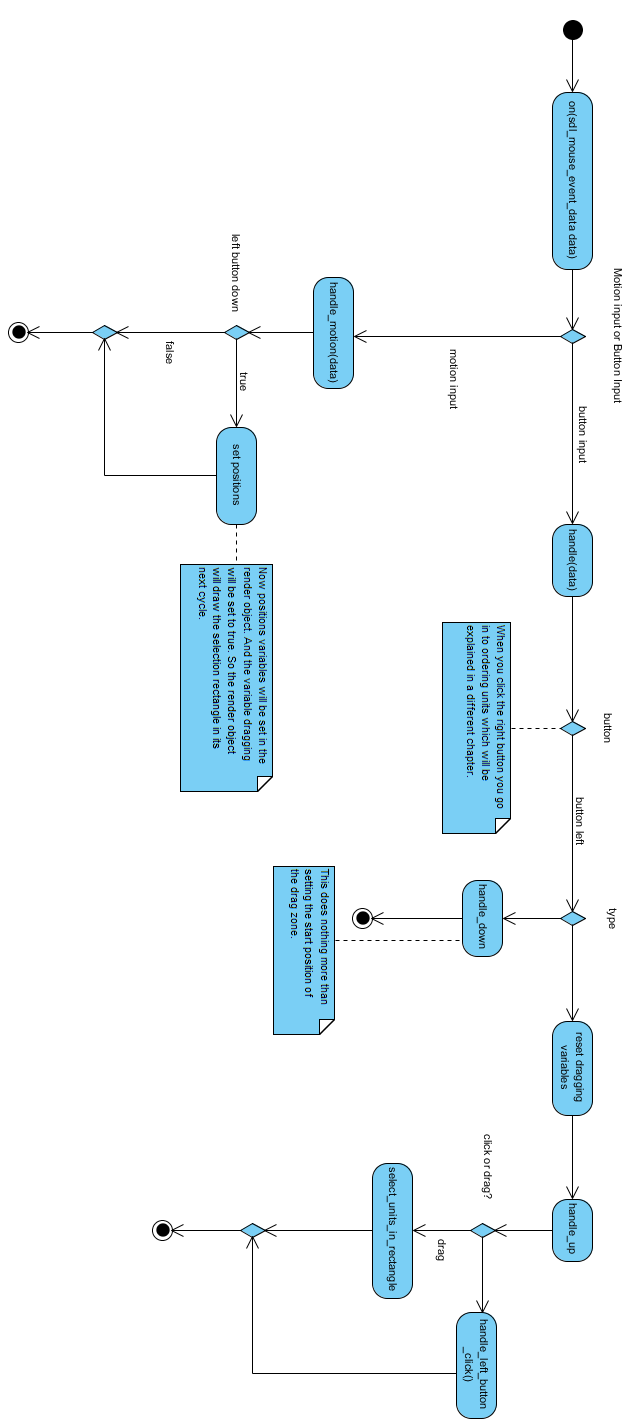
\includegraphics[scale=0.8]{res/ActivityDiagramMouseHandler180.png}
    \caption{Handling user input activity diagram.}\label{fig:activitymousehandler}
\end{figure}

\begin{figure}[!htb]
\centering
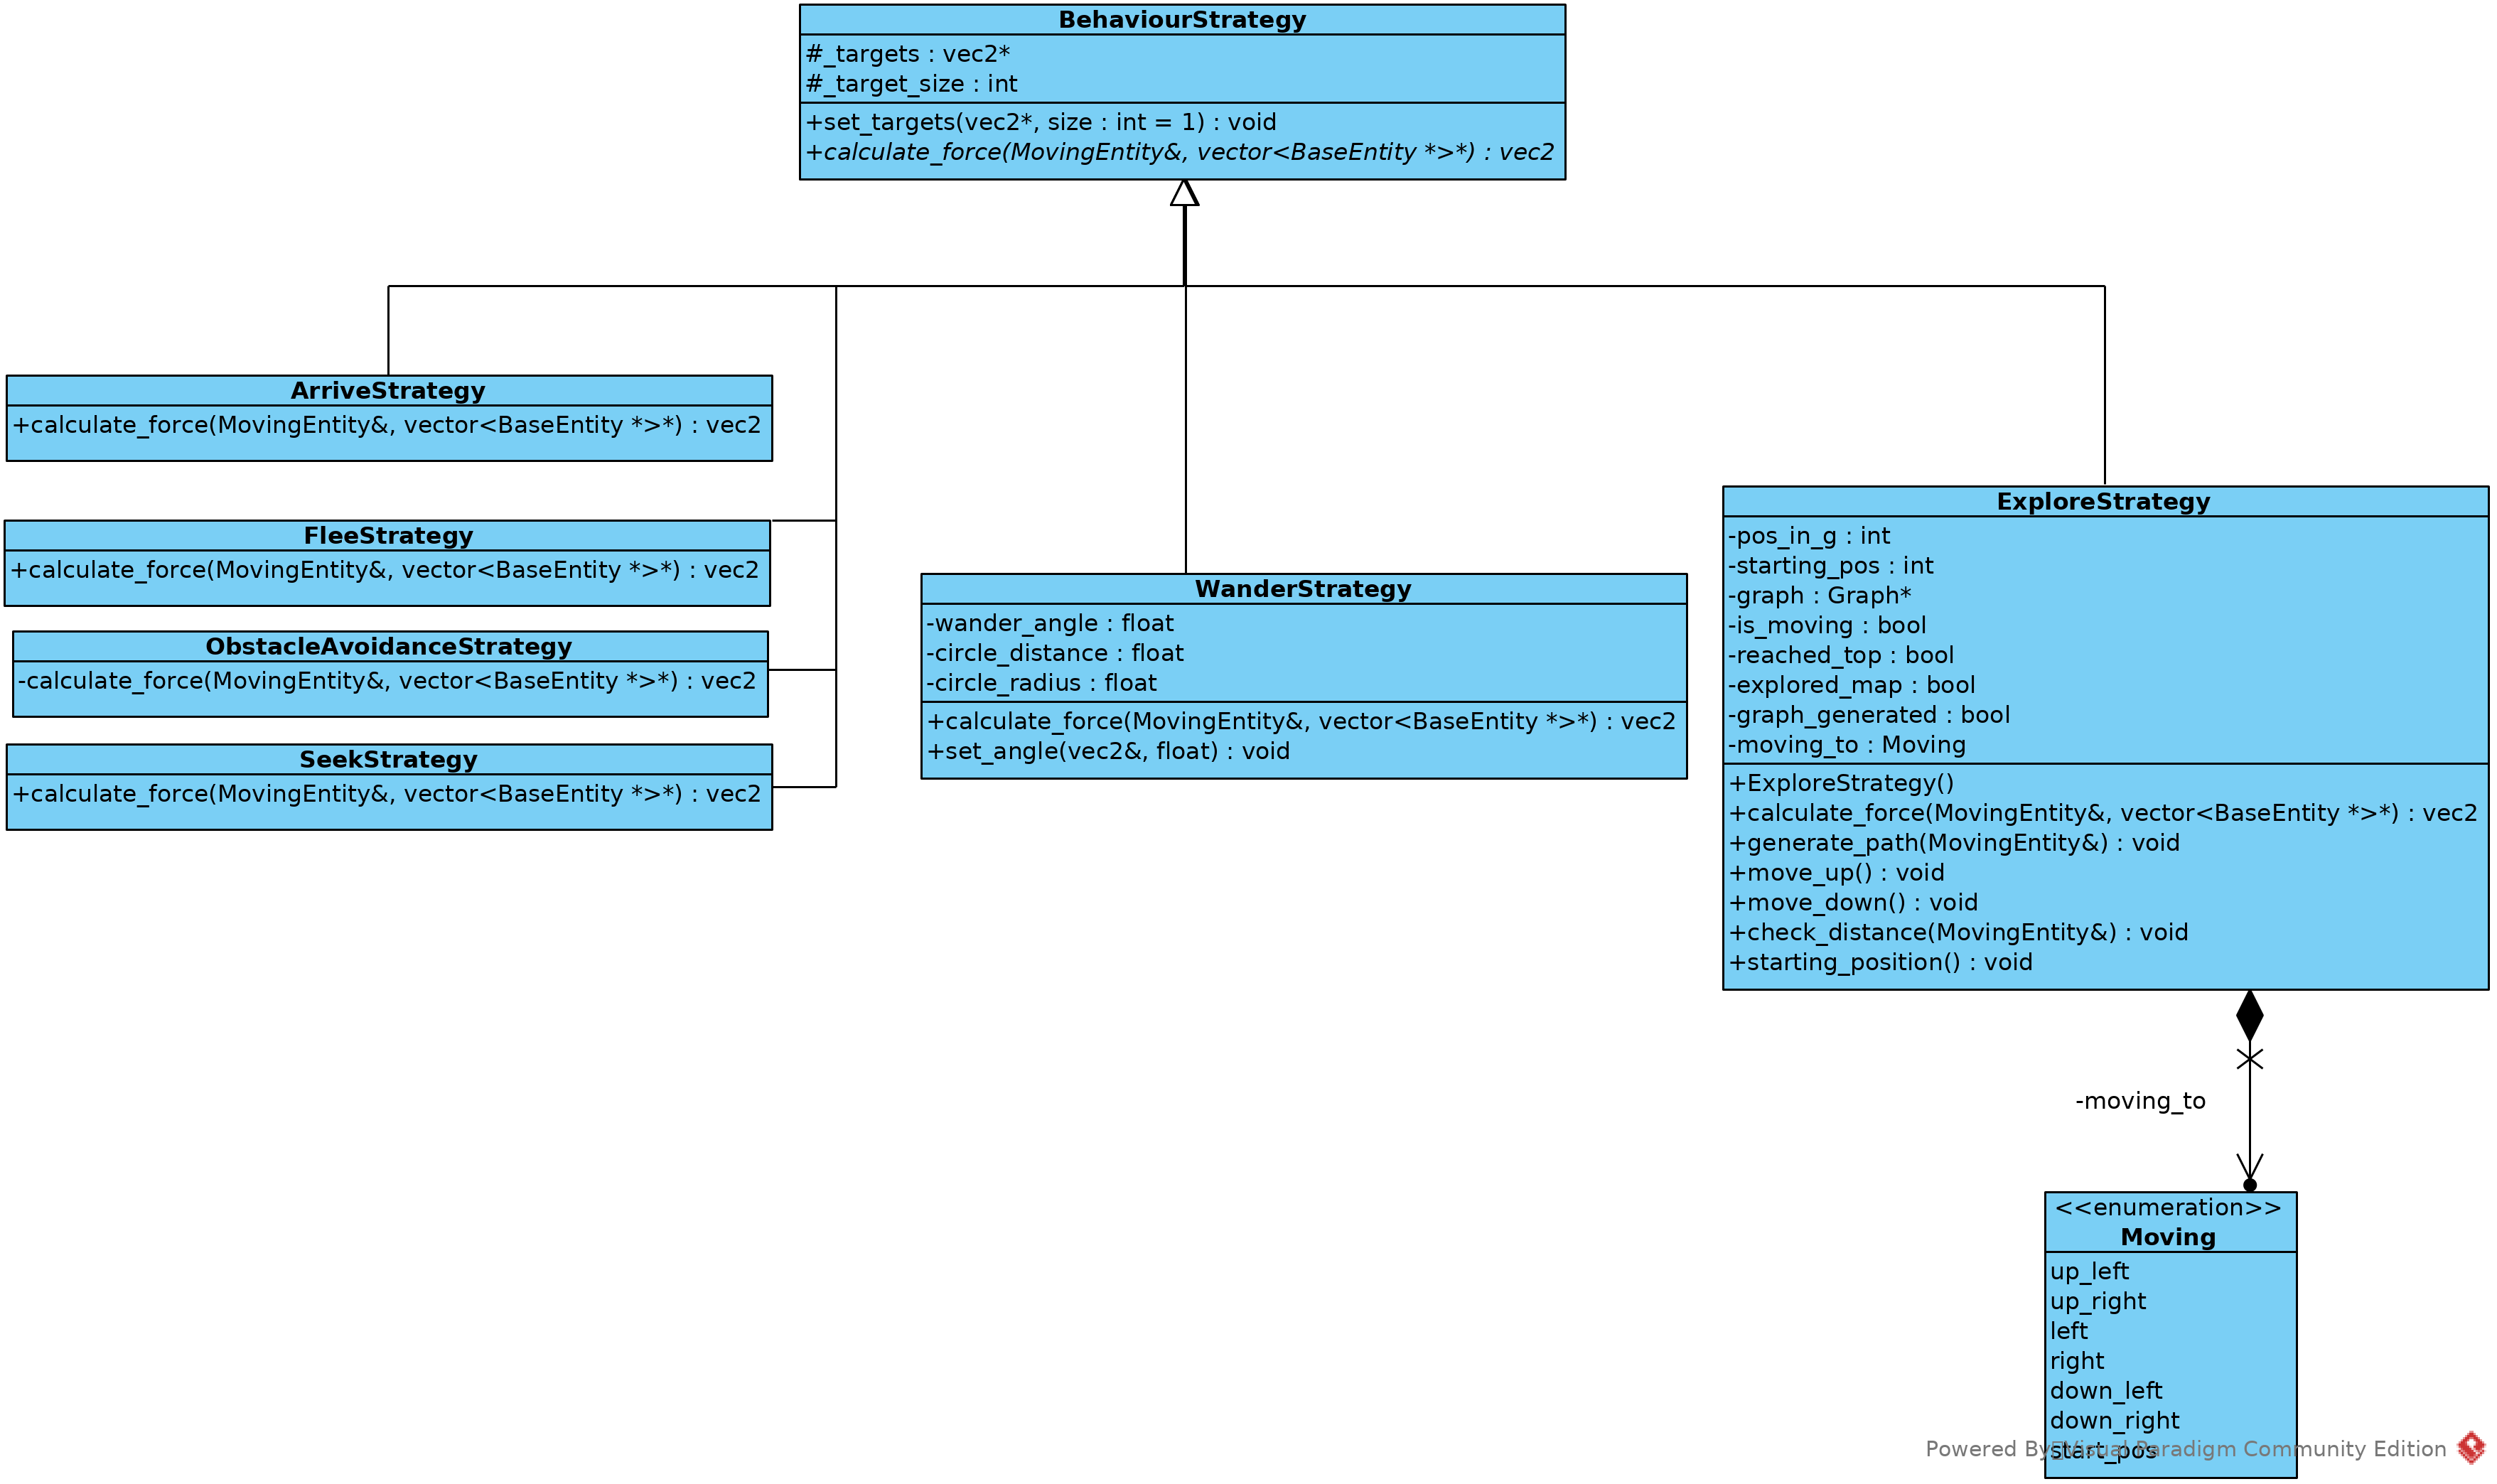
\includegraphics[angle=-90,origin=c,scale=0.6]{res/steering/BehaviourStrategy.png}
\caption{BehaviourStrategy class.}\label{fig:behaviourstrategy}
\end{figure}

\begin{figure}[!htb]
    \centering
    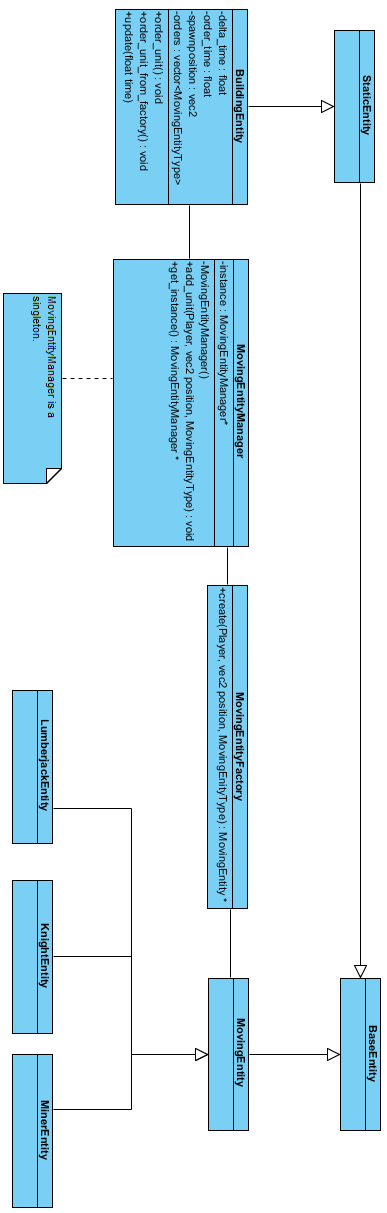
\includegraphics[scale=0.70]{res/MovingEntityFactoryClassRotated.png}
    \caption{Class structure around the MovingEntity factory.}
\end{figure}

\begin{figure}[!htb]
    \centering
    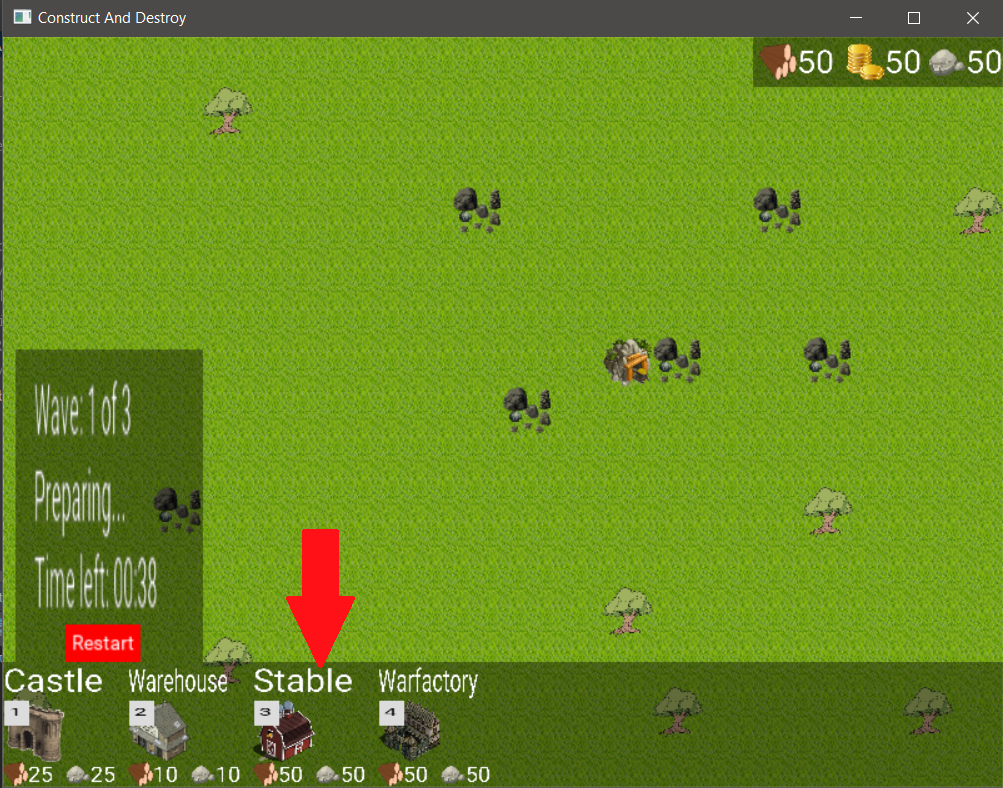
\includegraphics[scale=0.6]{res/building-panel.png}
    \caption{Building panel}\label{fig:building-panel}
\end{figure}

\begin{figure}[!htb]
    \centering
    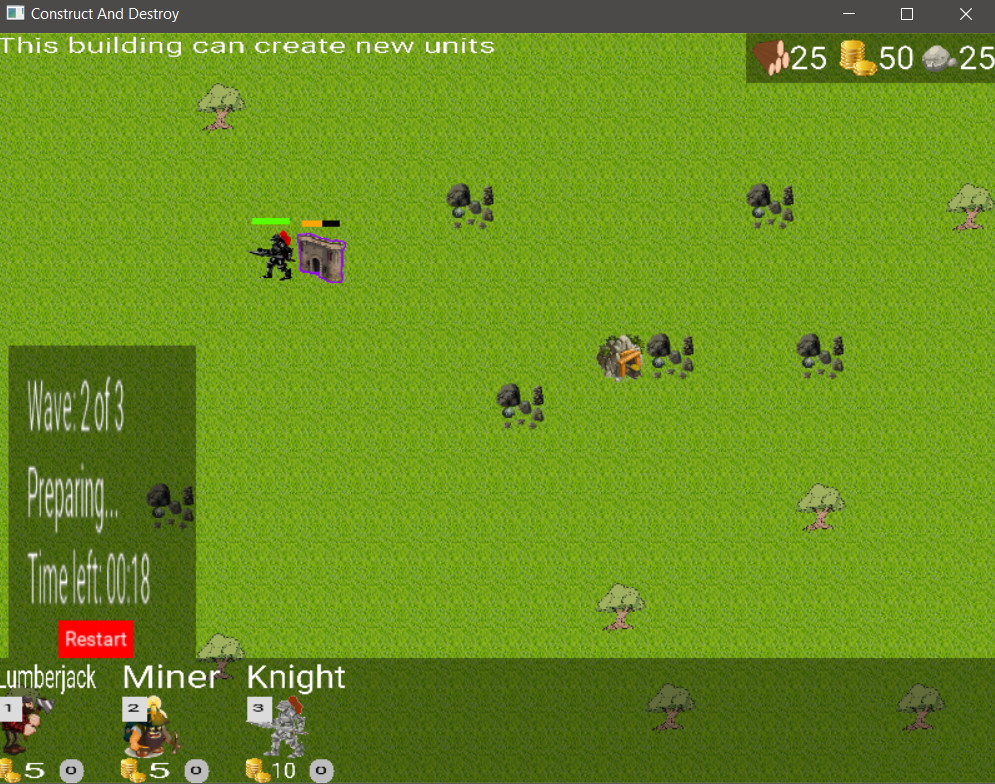
\includegraphics[scale=0.6]{res/entity-panel.png}
    \caption{Entity panel}\label{fig:entity-panel}
\end{figure}

\begin{figure}[!htb]
    \centering
    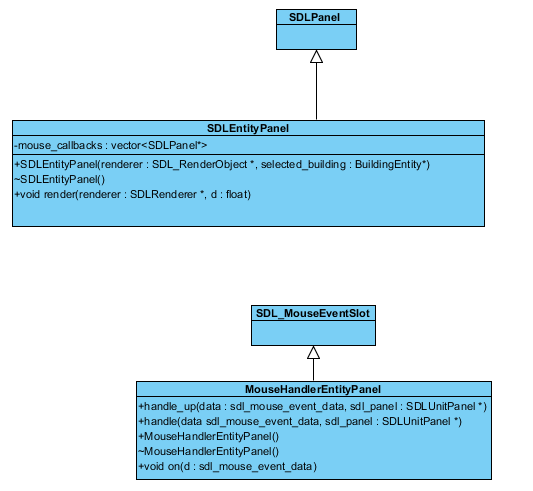
\includegraphics[scale=0.8]{res/entity-panel-class-diagram.png}
    \caption{Entity panel Class Diagram}\label{fig:entity-panel-class-diagram}
\end{figure}

\begin{figure}[!htb]
    \centering
    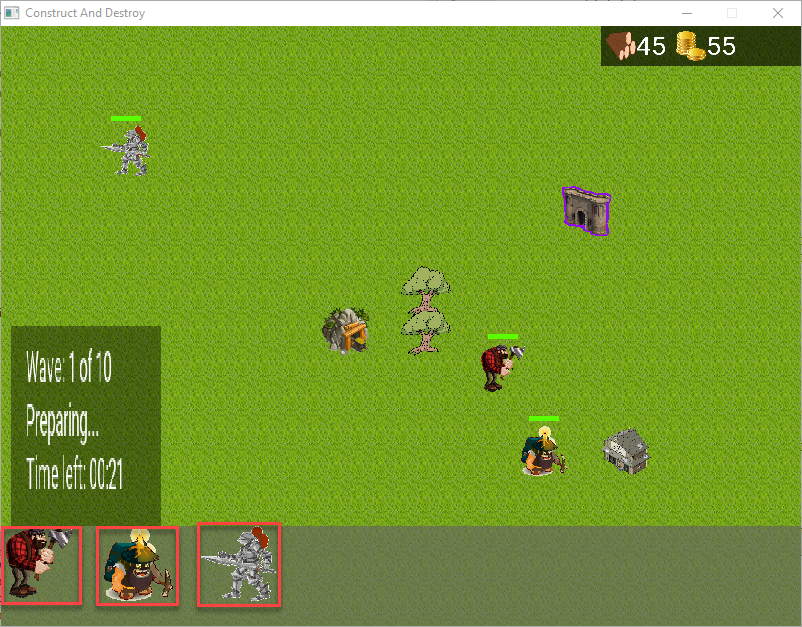
\includegraphics[scale=0.8]{res/unit-panel.png}
    \caption{Three unit panels}\label{fig:unit-panel}
\end{figure}

\begin{figure}[!htb]
    \centering
    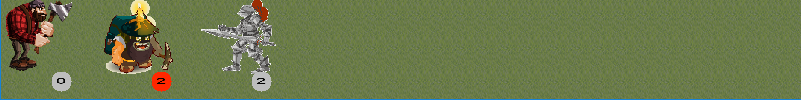
\includegraphics[scale=0.8]{res/unit-panel-order-queue.png}
    \caption{Order queue}\label{fig:unit-panel-order-queue}
\end{figure}

\begin{figure}[!htb]
    \centering
    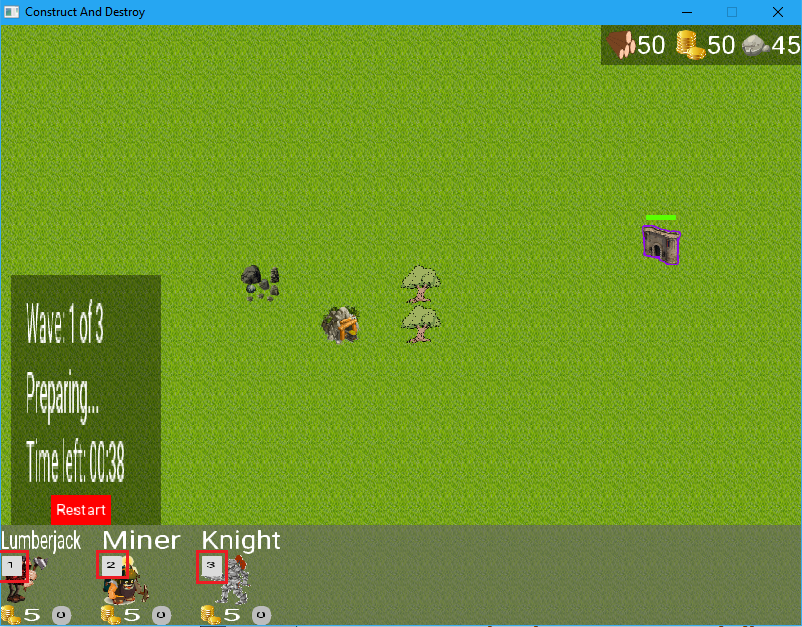
\includegraphics[scale=0.6]{res/entity-shortcuts.png}
    \caption{Entity shortcuts}\label{fig:entity-shortcuts}
\end{figure}

\begin{figure}[!htb]
    \centering
    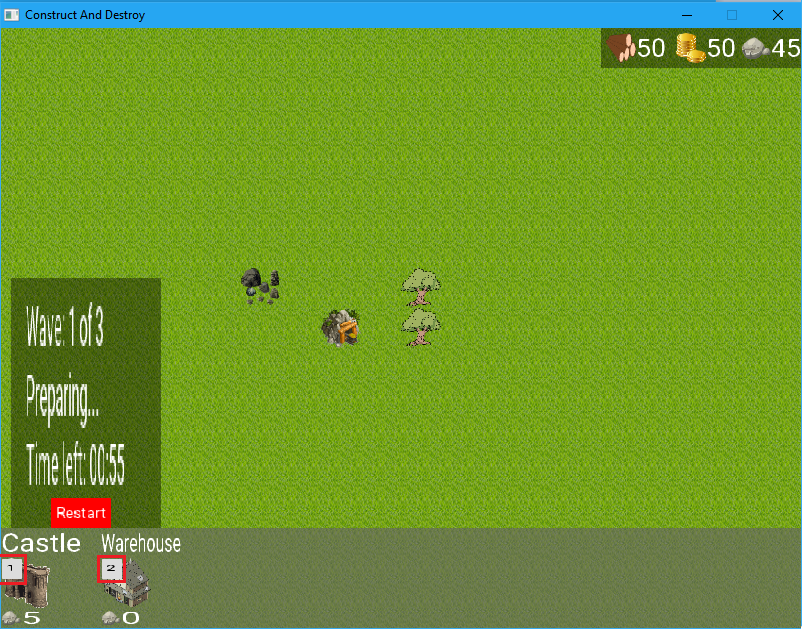
\includegraphics[scale=0.6]{res/building-shortcuts.png}
    \caption{Building shortcuts}\label{fig:building-shortcuts}
\end{figure}

\begin{figure}[!htb]
    \centering
    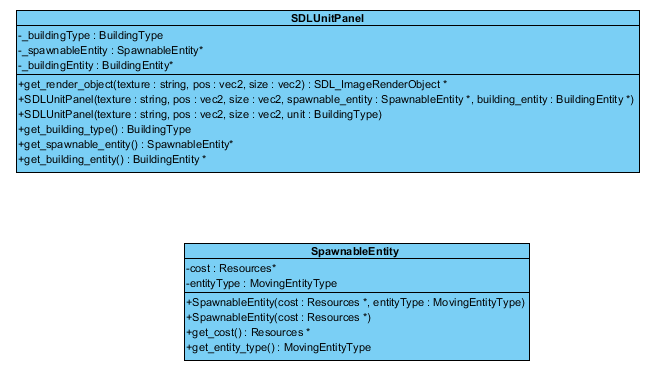
\includegraphics[scale=0.8]{res/unit-panel-class-diagram.png}
    \caption{Unit panel Class Diagram}\label{fig:unit-panel-class-diagram}
\end{figure}

\begin{figure}[!htb]
    \centering
    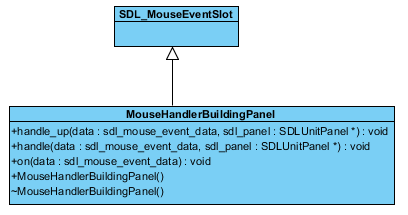
\includegraphics[scale=0.8]{res/mousehandlerbuildingpanel.png}
    \caption{Mouse handler building panel}\label{fig:mousehandlerbuildingpanel}
\end{figure}

\section{Conventions}
\subsection{Code conventions}
In this subsection we will give insights in the code conventions that our code must conform to. We will be using the GNU code conventions mainly, with some small adjustments.
The most common examples will be explained in this subsection. For more information about the GNU code conventions we would like to reference to the GCC Wiki-page. \cite{gccwcc}
\subsubsection{Variable names}
\paragraph{Snake casing functions and variables}
~\\Functions and variable names will start with a lower case. If the function or variable contains two or more words, these words will be separated with an underscore.

\textbf{Example function name:} \lstinline{this_is_a_function_name()}
~\\\textbf{Example variable name:} \lstinline{int variable_name;}

\paragraph{Constants uppercase}
~\\Constant variables are uppercase and separated with a underscore if it contains multiple words.

\textbf{Example constant variable name:} \lstinline{int MAX_SPEED = 10;}

\subsubsection{Class names}
Class names will be, opposite of variable names, PascalCase.

\textbf{Example class name:} \lstinline{class Agent}\clearpage

\subsubsection{Brackets}
We have chosen to use brackets where possible. We will put brackets on the same line as the class name, if-statement et cetera. The ending bracket will be on a new line.
If there is an else or else-if condition, the keyword will be on the ending bracket of the previous condition.

\textbf{Example brackets class declaration:}
\begin{lstlisting}
class Agent {
...
};
\end{lstlisting}

\textbf{Example brackets if...else-statement:}
\begin{lstlisting}
if(current_speed > agent->max_speed) {
...
} else {
... 
}
\end{lstlisting}

\subsubsection{Comments}
We decided we should not put unnecessary comments in our code. We strive for method and variable names that speak for themselves. If we place comments, we put them above a method, line of code or code block.

\textbf{Example correct comments:}
\begin{lstlisting}
...
// Calculate radius from input
var radians = input * 180.0 / M_PI;
...
\end{lstlisting}

\textbf{Example incorrect comments:}
\begin{lstlisting}
// Sum two integers
int sum_two_ints(int a, int b) {
	return a + b; // return a + b
};
\end{lstlisting}
